\documentclass[11pt]{article}
\usepackage[margin=1in]{geometry}
\usepackage[T1]{fontenc}
\usepackage{amsmath,amssymb}
\usepackage{microtype}
\usepackage{pgfplots}
\usepackage{listings}
\usepackage{graphicx}
\pgfplotsset{compat=1.18}
\usepackage[hidelinks]{hyperref}
\title{Chaos and Fractals: Patterns from Simple Rules}
\author{Hartwell Markham, Rob Tompkins, Rekik Ziku}
\date{\today}

\begin{document}
\maketitle

\begin{abstract}
This project explores how simple repeated rules can produce intricate patterns, connecting the study of chaos with the
geometry of fractals.
Chaos concerns systems whose behavior can become difficult to predict because small differences in their starting
conditions grow over time, while fractals describe shapes and sets with detail at increasingly small scales.
These ideas often meet, but fractal structure does not by itself imply chaotic behavior.
Using Chapter~11 of Strogatz's \emph{Nonlinear Dynamics and Chaos} as a foundation, we will consider how mathematicians
describe the size and complexity of such patterns through countability, uncountability, and fractal dimension.
The Cantor set provides a central example: removing intervals repeatedly leaves an uncountable collection of points with
zero total length.
Box dimension offers another way to understand its size by tracking how many small boxes are needed to cover it as the
scale becomes finer.

Two examples will connect these abstract ideas to the emergence of recognizable patterns: the chaos game and the Devil's
staircase.
In the familiar chaos game, repeatedly moving partway toward a randomly chosen vertex of a triangle produces the
Sierpi\'nski triangle, showing how random choices can reveal an organized geometric structure.
Barnsley and Vince's \emph{The chaos game on a general iterated function system} explains why this approach can recover
an attracting set under broad conditions, extending beyond the usual setting in which every rule shrinks distances.
Per Bak's \emph{The Devil's staircase} examines a different source of intricate organization: systems with competing
rhythms that synchronize over ranges of conditions, creating a hierarchy of plateaus separated by a Cantor-like set.
Together, these examples frame the project around a shared question: how does repeated evolution produce structure
across scales?
By comparing a fractal generated by random iteration with fractal organization among the conditions for synchronization,
we will use visual examples and accessible geometric ideas to connect unpredictability, order, and the different
meanings of mathematical size.

\end{abstract}

\section{Random iteration: the circle attractor}

We've used both python and matlab to reproduce Example~1 of Barnsley and Vince
\cite{barnsley-vince}, we take the state space to be the unit circle
and at each step independently choose either the identity or a rotation, each with probability $1/2$.
We use the irrational rotation angle $2\pi(\sqrt{5}-1)/2$ and start at $(1,0)$.
Both maps preserve distances, so this example tests the chaos game beyond the familiar contracting maps that
generate the Sierpi\'nski triangle.

Write the circle as $\mathbb T=\mathbb R/\mathbb Z$ and let $\alpha=(\sqrt5-1)/2$.
From phase $t_0$, the set of all $n$-step images is $\{t_0+j\alpha:0\le j\le n\}$ modulo one.
The forward orbit of an irrational rotation is dense, and compactness implies that some finite prefix is an
$\varepsilon$-net for each $\varepsilon>0$.
For any nonempty compact initial set $B$ on the circle, the $n$-step images of $B$ contain the images of a
single point of $B$ and lie on the circle, so their Hausdorff limit is the circle as well.

In the random experiment let $S_n$ count rotations among the first $n$ choices.
The phase at step $n$ is $t_0+\alpha S_n$ modulo one, and the strong law gives $S_n/n\to1/2$ almost surely.
Because the count increases by zero or one, every tail visits all rotation counts from its starting count onward.
Thus every tail is dense almost surely, even though two starting phases driven by the same choices stay the
same distance apart.
Attraction describes the coverage by sets of images here; individual trajectories need not approach one another.

For a finite set of sampled points, let $g_N$ denote the largest gap between successive distinct phases, measured
in turns and including the wraparound gap.
The point farthest from the sample is at the midpoint of that gap, so the Euclidean Hausdorff distance to the circle is
\[
d_H = 2\sin(\pi g_N/2).
\]
The midpoint of the largest gap is at angular distance $\pi g_N$ from its nearest sample, and the
corresponding chord has length $2\sin(\pi g_N/2)$.
The reverse directed distance is zero because every sample point lies on the circle.
If there are $M$ distinct phases, the gaps sum to one, so $g_N\ge1/M$.
Thus $2\sin(\pi/(2M))$ is the best possible coverage error for $M$ samples, attained by equal spacing.

The experiment uses a fixed random seed and measures cumulative coverage at powers of two.
The error drops from $1.129$ after $8$ iterates to $0.00230$ after $4096$.
Figure~\ref{fig:circle} reproduces the qualitative finding that a single random orbit draws the circle and adds a
numerical measure of how well the sample covers it.
The finite prefix calculation illustrates coverage; the almost sure statement about infinite tails comes from
the argument above and the theorem, rather than the plot.

\begin{figure}[htbp]
\centering
\begin{tikzpicture}
\begin{axis}[width=.40\linewidth,height=5cm,axis equal image,xmin=-1.15,xmax=1.15,ymin=-1.15,ymax=1.15,
  xlabel={$x$},ylabel={$y$},title={First 512 iterates}]
\addplot[only marks,mark=*,mark size=.62pt,blue!65!black]
  table[col sep=comma,x=x,y=y]{data/circle.csv};
\end{axis}
\end{tikzpicture}
\hfill
\begin{tikzpicture}
\begin{loglogaxis}[width=.49\linewidth,height=5cm,xlabel={Iterates $N$},ylabel={Hausdorff distance},
  title={Coverage error},grid=major]
\addplot[blue!65!black,mark=*] table[col sep=comma,x=n,y=distance]{data/coverage.csv};
\end{loglogaxis}
\end{tikzpicture}
\caption{The noncontractive chaos game on the unit circle.
Repeated points do not improve coverage; newly visited phases close the gaps.}
\label{fig:circle}
\end{figure}

\section{Frequency locking: the critical Devil's staircase}

To reproduce the winding number staircase in Figure~5(c) of Bak \cite{bak}, we iterate the lift of the sine circle map,
\[
x_{n+1}=x_n+\Omega+\frac{K}{2\pi}\sin(2\pi x_n).
\]
The bias $\Omega$ is the uncoupled advance per step, and $K$ sets the strength of the periodic term.
At the critical value $K=1$, we estimate the winding number by averaging the unwrapped increments after a transient.
The implementation keeps the phase modulo one for evaluating the sine but accumulates the full increments.
We use $3001$ equally spaced values of $\Omega$ on $[0,1]$, discard $4096$ steps and average the next $16384$,
starting all runs at phase $0.123$.

\subsection{Existence of the winding number and mechanism of locking}

Write $F_\Omega$ for the lift at $K=1$.
It is increasing because $F_\Omega'(x)=1+\cos(2\pi x)\ge0$ and the zeros of the derivative are isolated.
It satisfies $F_\Omega(x+1)=F_\Omega(x)+1$.
Let $D_n(x)=F_\Omega^n(x)-x$, and let $a_n$ and $b_n$ be its minimum and maximum over one period.
For $x\le y\le x+1$, the difference $F_\Omega^n(y)-F_\Omega^n(x)$ lies in $[0,1]$, so $b_n-a_n\le1$.
The identity $D_{n+m}(x)=D_n(x)+D_m(F_\Omega^n(x))$ makes $a_n$ superadditive and $b_n$ subadditive.
By the superadditive and subadditive limit lemmas, their normalized limits coincide, giving a common winding
number $W$ for every initial phase.
Moreover, $a_n\le nW\le b_n$, so $|D_n(x)/n-W|\le1/n$ for any starting phase.
For $16384$ iterates this bounds the finite-window error by $6.11\times10^{-5}$ in exact arithmetic.
Increasing $\Omega$ increases the lift pointwise, so monotonicity of the iterates makes $W$ nondecreasing.

If $F_\Omega^q(x_*)=x_*+p$, then $F_\Omega^{mq}(x_*)=x_*+mp$ for every positive integer $m$, giving $W=p/q$.
A root of $F_\Omega^q(x)-x-p=0$ persists as $\Omega$ varies locally whenever the cycle multiplier
$\lambda=(F_\Omega^q)'(x_*)$ differs from one, by the implicit function theorem.
By the chain rule this multiplier is the product of the $q$ derivatives along the cycle, and
$0\le\lambda<1$ gives local attraction.
At $\Omega=1/2$, the lift sends $0$ to $1/2$ and then to $1$, giving $W=1/2$ and
$\lambda=(1+\cos 0)(1+\cos\pi)=0$.
The resulting persistence of this period-two orbit explains why the central step has positive width.

\subsection{Comparison with the numerical sweep}

Figure~\ref{fig:staircase} shows broad plateaus at $0$, $1/2$ and $1$, with smaller steps including $1/3$ and $2/3$.
For example, the computed winding number is within $2\times10^{-5}$ of $1/2$ at grid points from $0.463333$ to
$0.536667$.
This is a grid-based estimate, not a determination of the exact plateau endpoints.
The maximum change across the grid when doubling both the transient and averaging windows from half their final
values was $5.51\times10^{-5}$.
As a separate check, a fixed point of the lift satisfies $\Omega=-\sin(2\pi x)/(2\pi)$ at $K=1$.
Thus the zero-winding plateau on $[0,1]$ extends to $1/(2\pi)\approx0.159155$, consistent with the last detected
grid point at $0.159000$.
The finite grid resolves only some of the plateaus and cannot establish that the full staircase occupies full measure.

\begin{figure}[htbp]
\centering
\begin{tikzpicture}
\begin{axis}[width=.53\linewidth,height=5cm,xmin=0,xmax=1,ymin=-.03,ymax=1.03,
  xlabel={Bias $\Omega$},ylabel={Winding number $W$},grid=major,legend pos=north west]
\addplot[blue!65!black,thick,no marks] table[col sep=comma,x=bias,y=winding]{data/staircase.csv};
\addlegendentry{Critical coupling, $K=1$}
\addplot[gray,dashed,domain=0:1,samples=2]{x};
\addlegendentry{Uncoupled, $K=0$}
\end{axis}
\end{tikzpicture}
\IfFileExists{plots/matlab_staircase.png}{%
  \hfill
  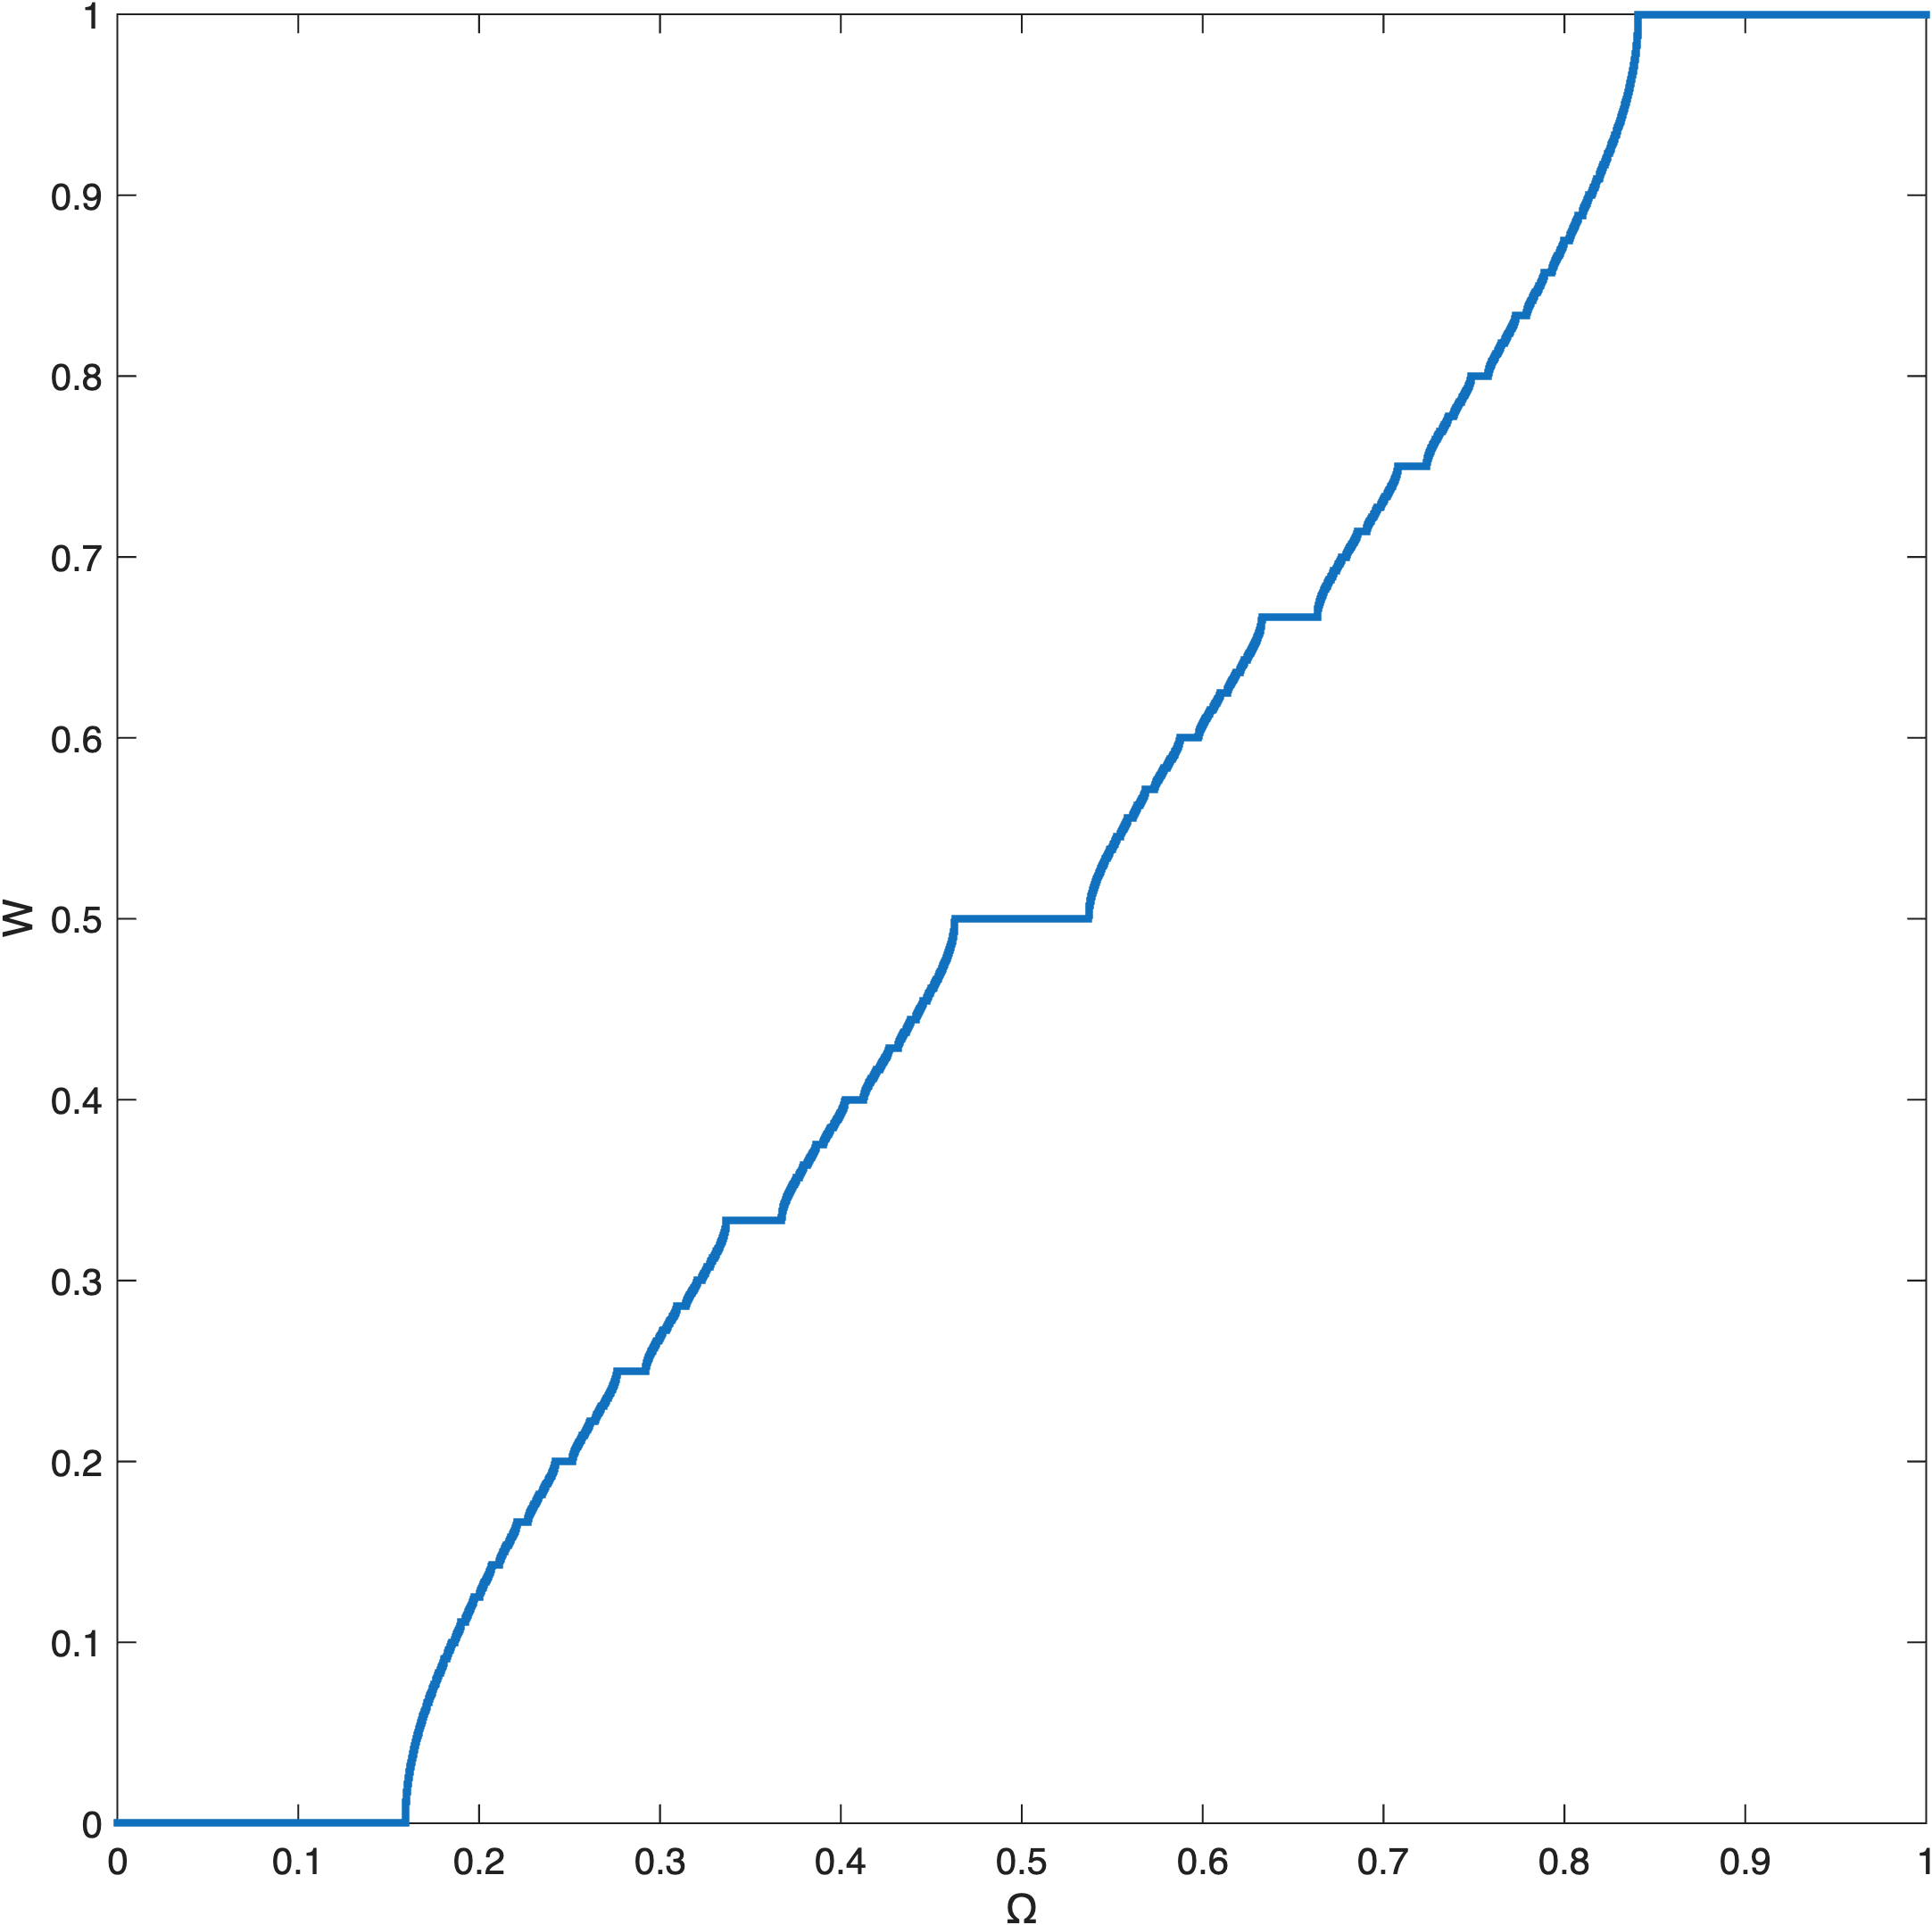
\includegraphics[width=.43\linewidth,height=5cm,keepaspectratio]{plots/matlab_staircase.png}%
}{}
\caption{Numerical reproduction of Bak's critical winding number staircase.
%
\IfFileExists{plots/matlab_staircase.png}{%
  The Python/TikZ plot is on the left and the MATLAB export (\texttt{matlab\_staircase.png}) is on the right.
}{}
Horizontal segments indicate that the same average rotation persists over a range of biases.}
\label{fig:staircase}
\end{figure}

\IfFileExists{plots/matlab_circle_map.png}{%
  \begin{figure}[htbp]
    \centering
    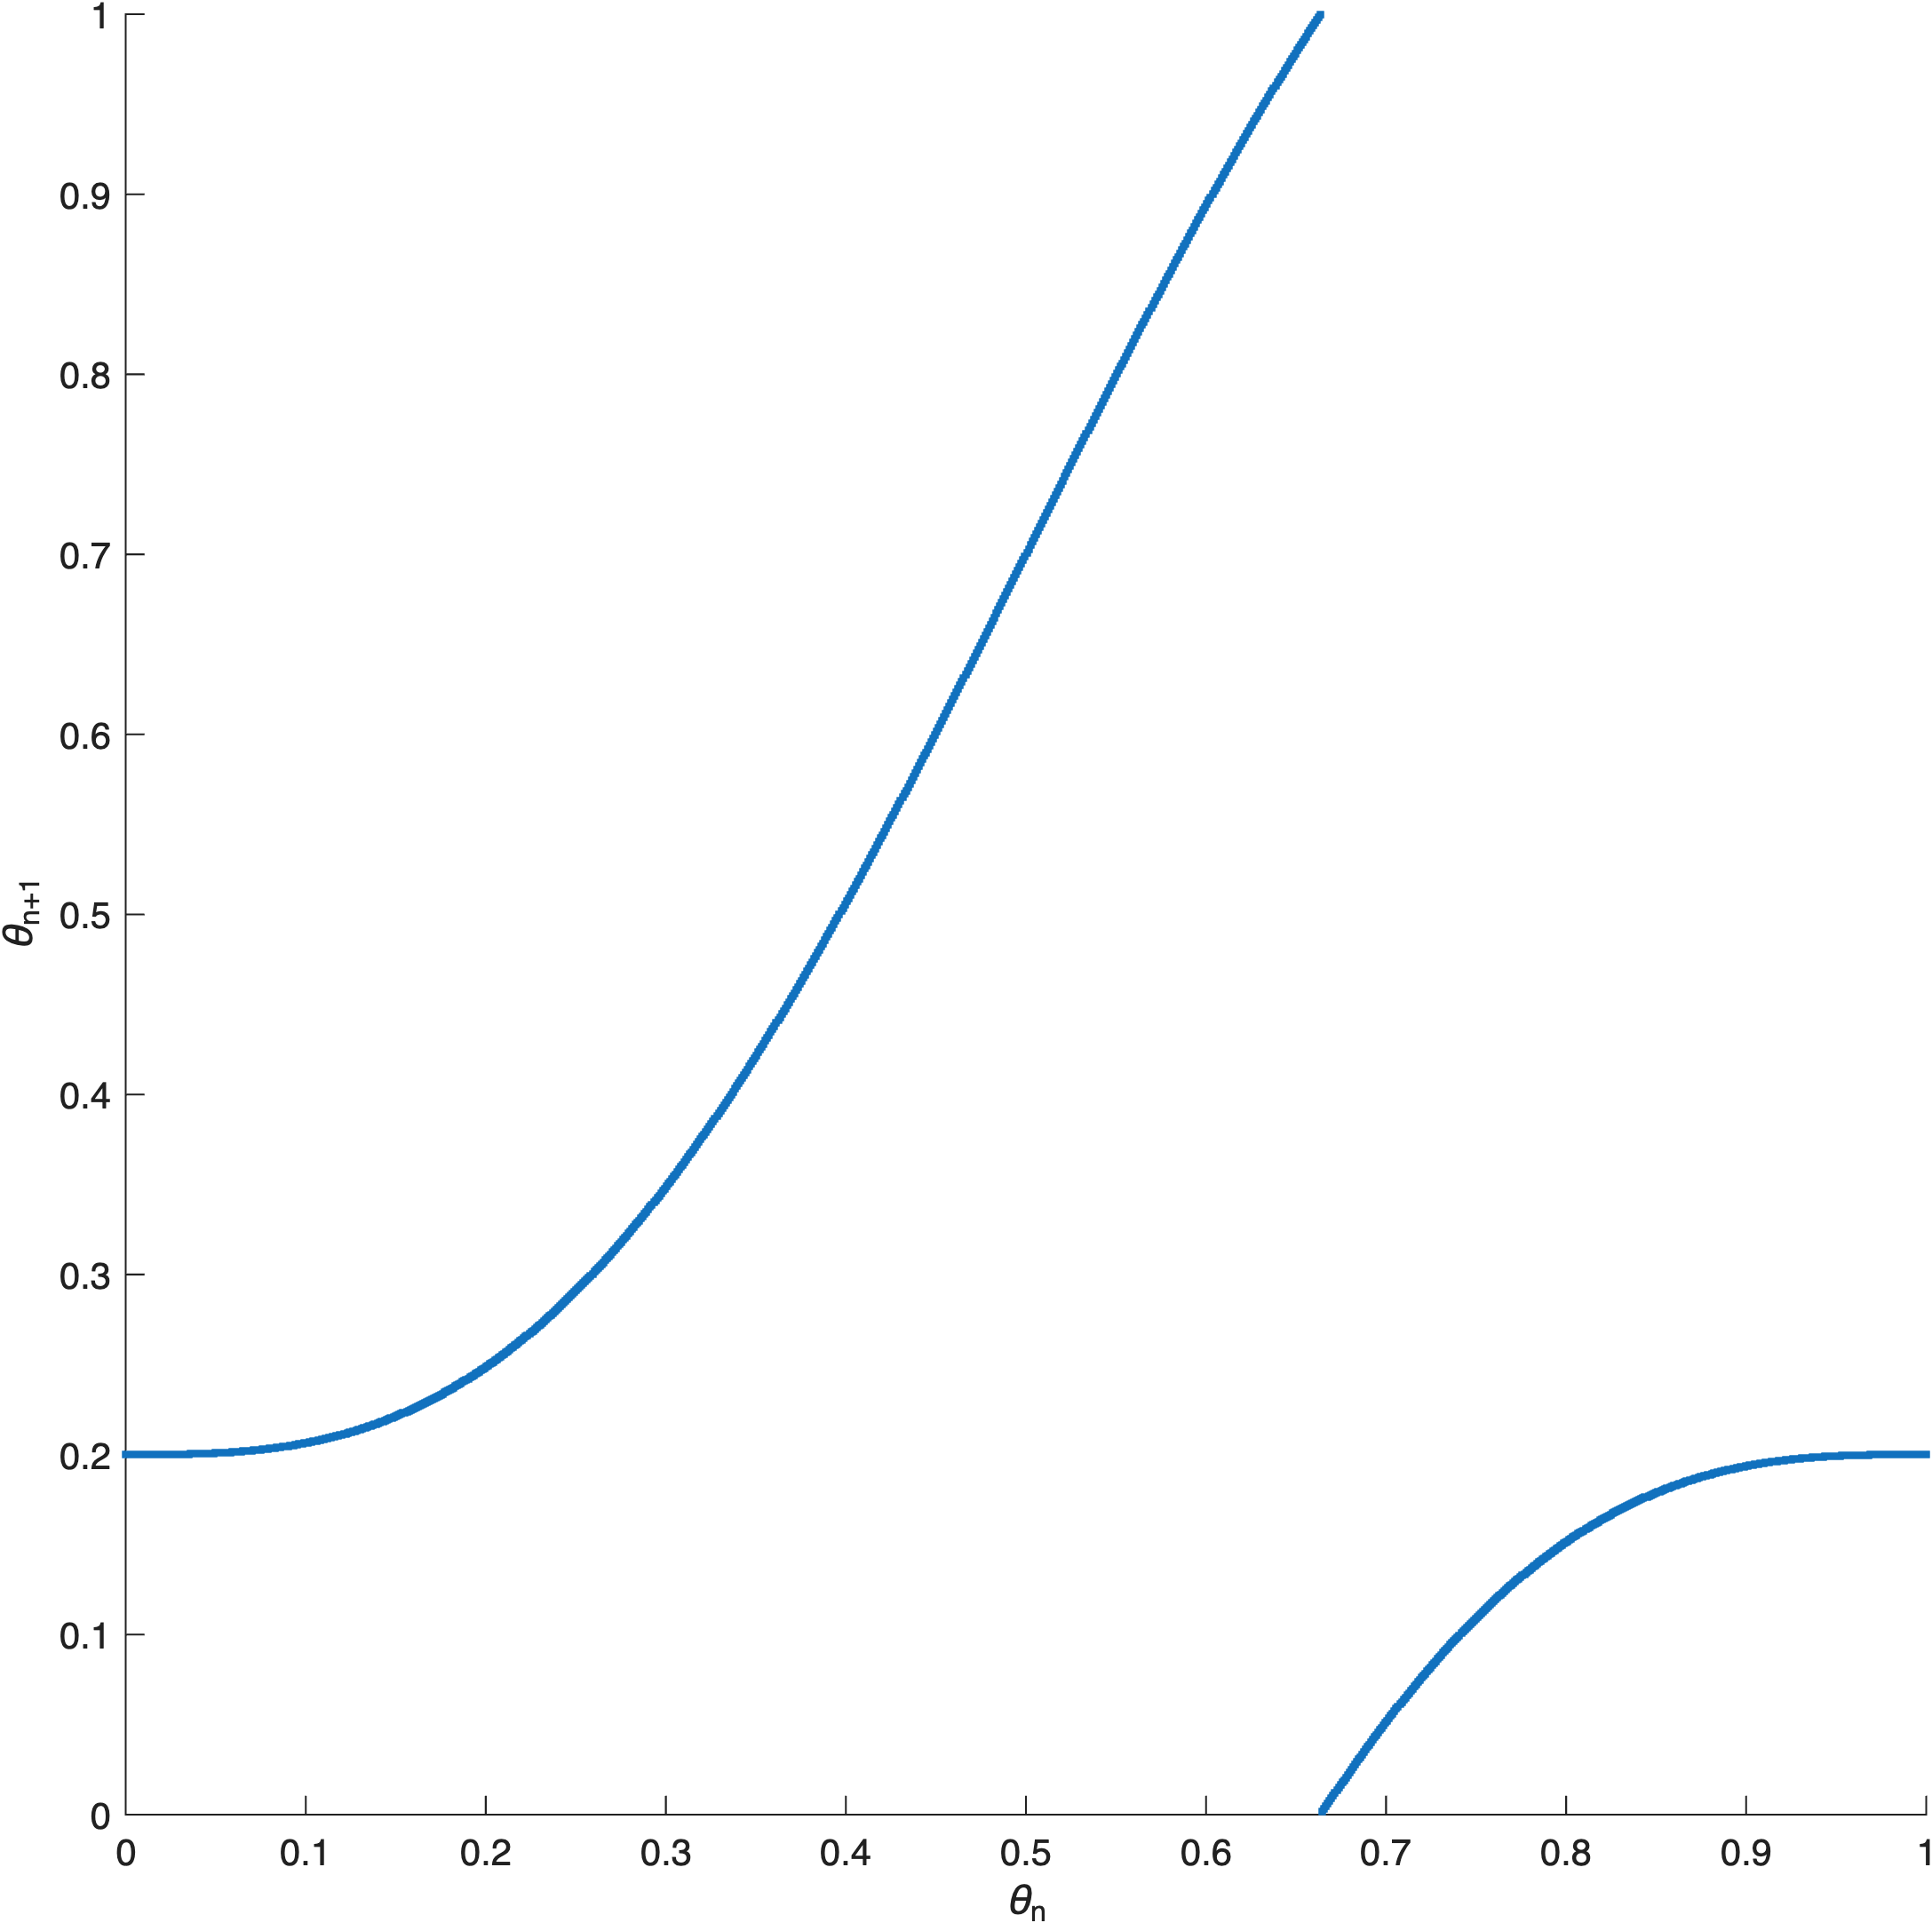
\includegraphics[width=.52\linewidth,height=5cm,keepaspectratio]{plots/matlab_circle_map.png}
    \caption{The MATLAB circle map (\texttt{matlab\_circle\_map.png}) at $\Omega=0.2$ and $K=1$.
    The graph shows one step modulo one for the map used to produce the staircase.}
    \label{fig:matlab-map}
  \end{figure}
}{}

\section{The connection through fractal dimension}

Strogatz \cite[Chapter~11]{strogatz} distinguishes counting points, measuring length, and counting boxes as
the observation scale shrinks.
For instance, the middle-thirds Cantor set has zero length and uncountably many points, yet at scale $3^{-m}$
it takes on the order of $2^m$ boxes to cover it, giving box dimension $\log 2/\log 3$.
These are three different ways to describe the same set.

The circle experiment concerns the geometry of an attractor in state space.
Its orbit has only countably many points, yet its closure is the entire circle, with box dimension one.
The staircase experiment concerns geometry in parameter space: its fractal set lies on the bias axis, where
the open locking intervals have been removed.
Bak estimates its dimension near $0.87$ by measuring how much of the bias axis remains uncovered after accounting
for plateaus wider than a scale $r$ and dividing the remaining length by $r$.
To make the connection precise, let $E$ be the closed set left after removing the open locking intervals
and include the endpoints of $[0,1]$.
In the complete staircase, $E$ has measure zero.
If its complementary gaps have lengths $\ell_j$, the length of the $r/2$-neighborhood of $E$ inside
$[0,1]$ is $V(r)=\sum_j\min(\ell_j,r)$.
Each gap wider than $r$ contributes two strips of length $r/2$, and each shorter gap contributes its full length.
Writing $L(r)$ for the number of gaps wider than $r$ and $S(r)$ for their total length gives
\[
\frac{V(r)}{r}=L(r)+\frac{1-S(r)}{r}.
\]
The ratio $V(r)/r$ is comparable up to constants to the number of mesh intervals of length $r$ meeting $E$.
The neighborhood lies in those intervals and their neighbors, and each occupied interval contains at least
$r/2$ of neighborhood length.
Bak fits the second term alone; the identity explains why it measures geometry at scale $r$ without being
literally the same as the mesh count.

The MATLAB experiment in Appendix~\ref{app:matlab} attempts the dimension calculation using widths
detected on a finite grid.
A fit on this grid alone does not verify Bak's dimension estimate.
The shared lesson is that a finite orbit or a finite parameter scan shows structure at a chosen resolution;
the limiting set explains what those observations are approaching.

\IfFileExists{plots/matlab_dimension_fit.png}{%
  \begin{figure}[htbp]
    \centering
    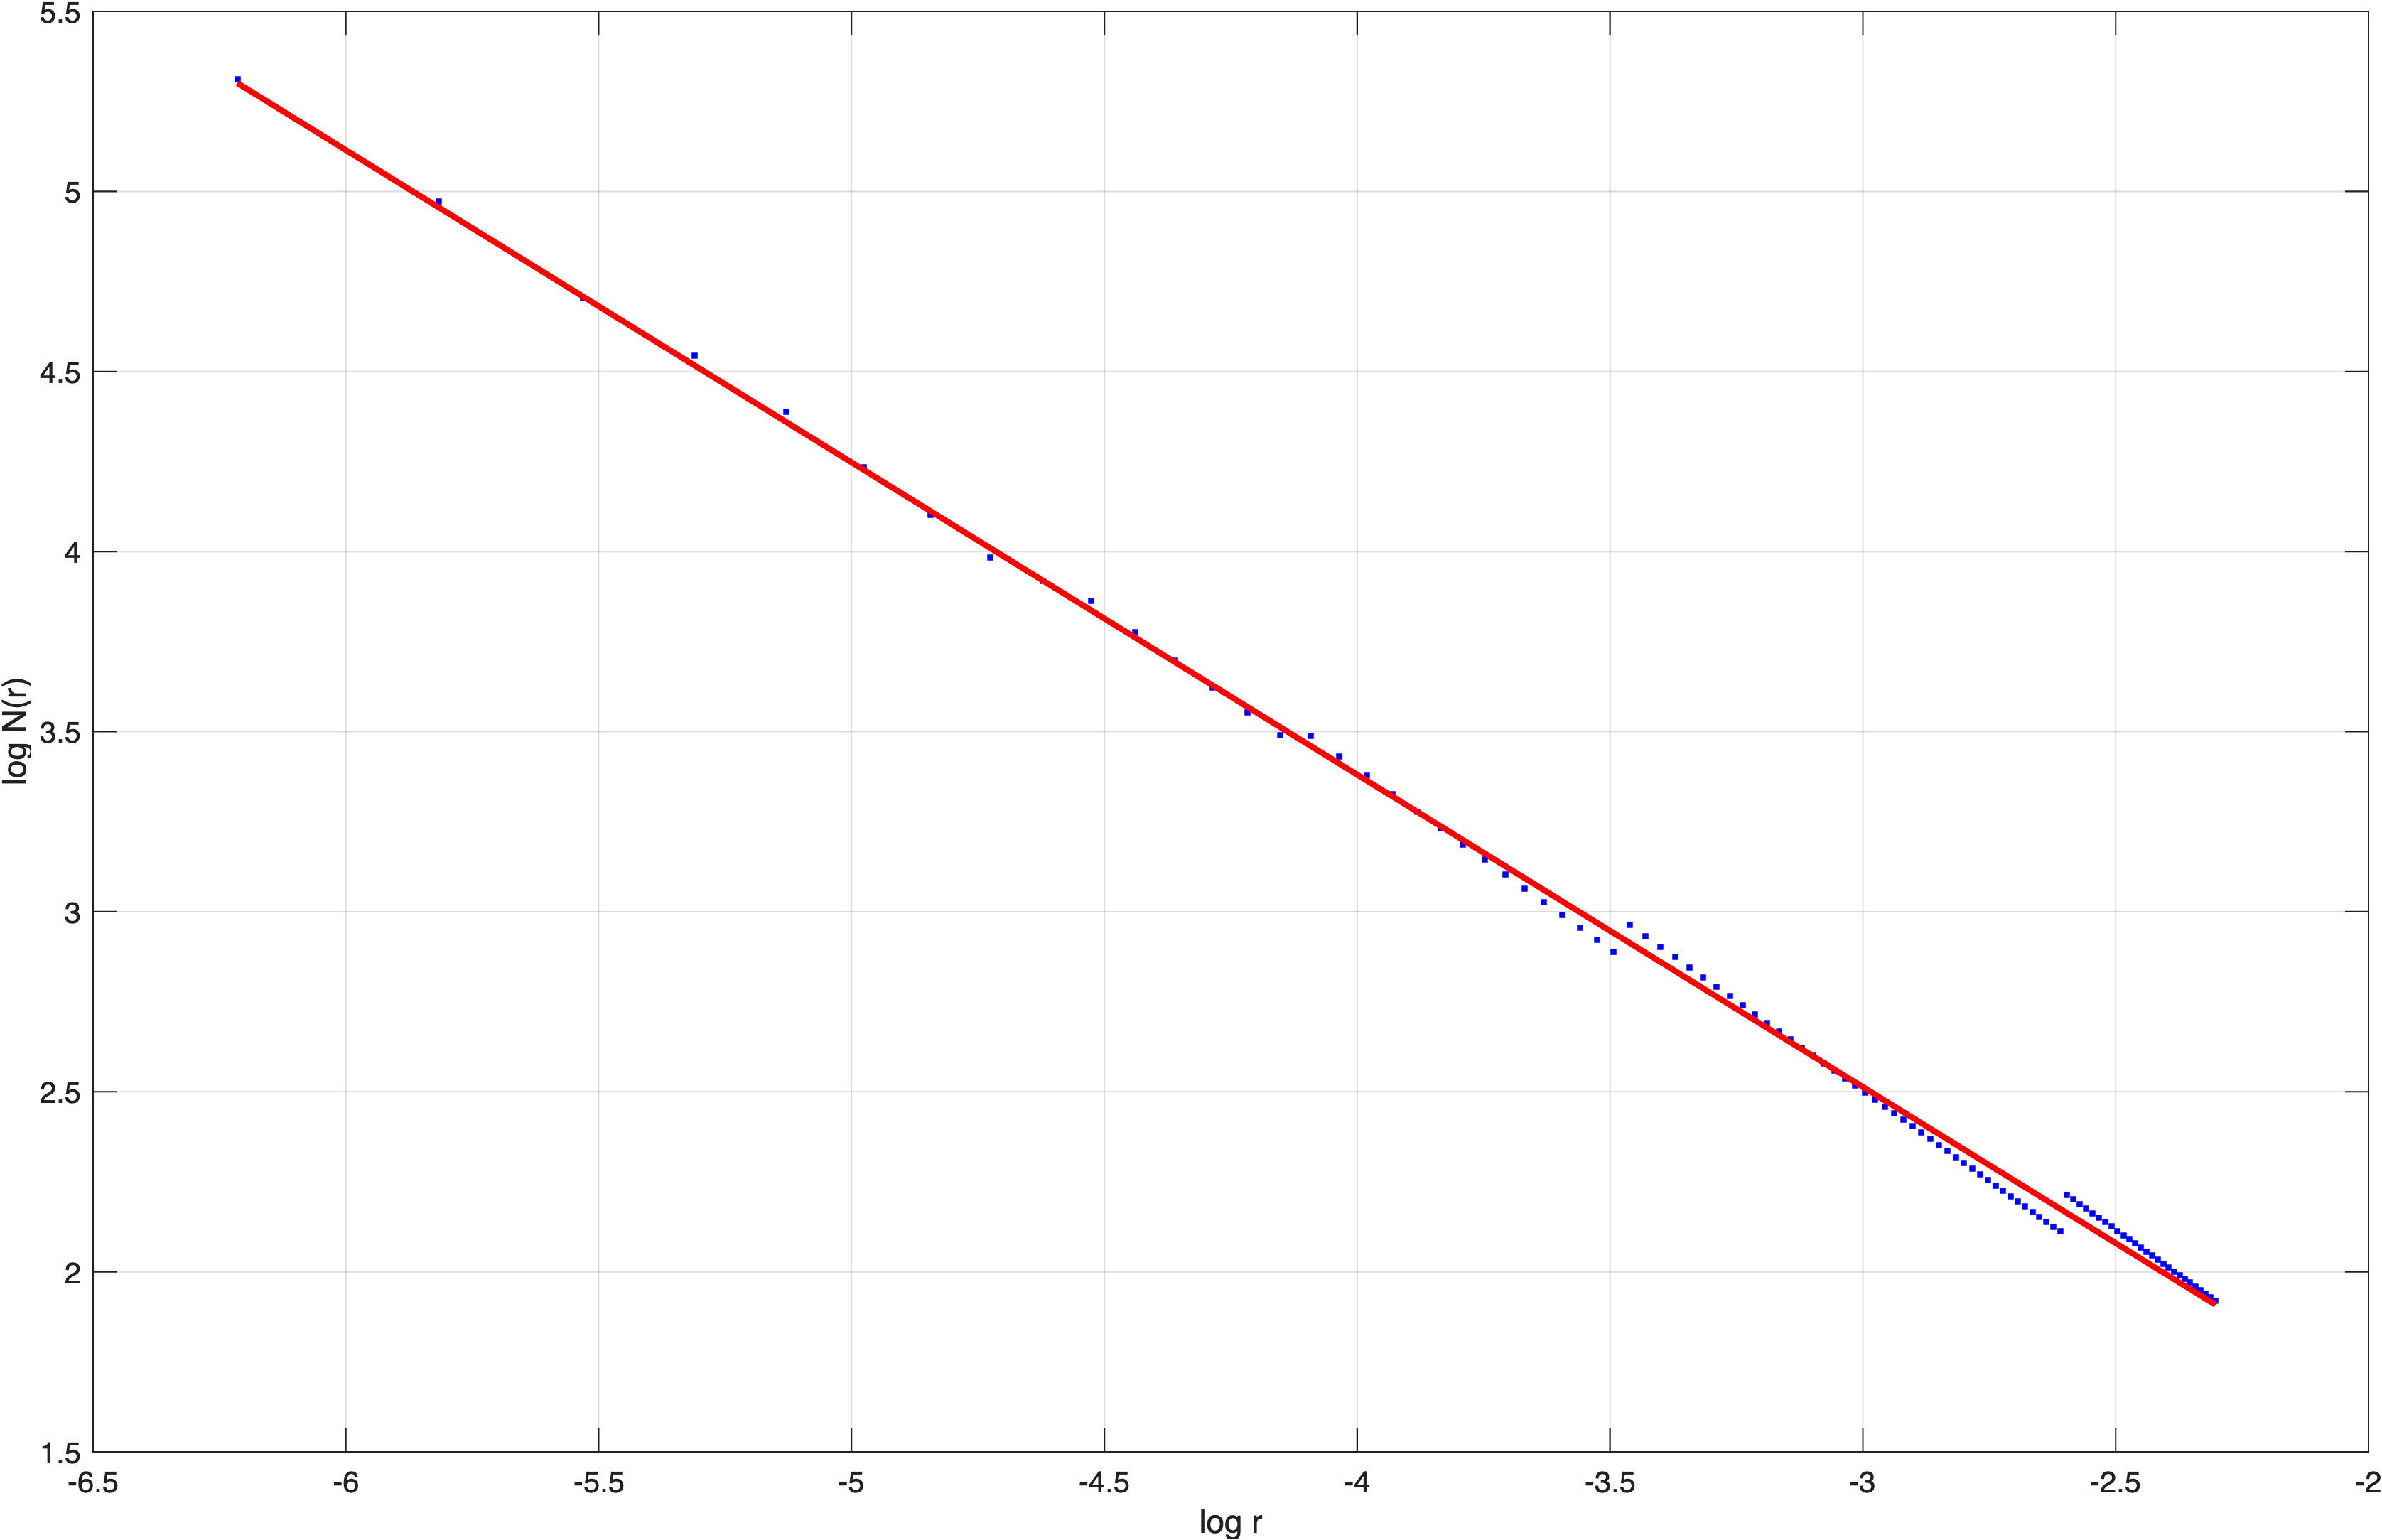
\includegraphics[width=.64\linewidth,height=5.5cm,keepaspectratio]{plots/matlab_dimension_fit.png}
    \caption{MATLAB fit of Bak's gap statistic (\texttt{matlab\_dimension\_fit.png}).
    The candidate dimension is the negative of the fitted slope.}
    \label{fig:matlab-dimension}
  \end{figure}
}{}

\paragraph{Code and figures.}
The files can be found in the
\href{https://github.com/chtompki/MathFall2026/tree/main/DynamicalSystems/ClassProjectPart2}{GitHub project directory}.
The source files are \texttt{chaos\_game.py}, \texttt{devil\_staircase.py}, and \texttt{circle\_map\_dimension.m}.
The \texttt{plots/} directory contains the Python previews \texttt{chaos\_game.png} and \texttt{devil\_staircase.png},
and the MATLAB exports \texttt{matlab\_circle\_map.png}, \texttt{matlab\_staircase.png}, and
\texttt{matlab\_dimension\_fit.png}.

\begin{thebibliography}{9}

\bibitem{strogatz}
Steven H. Strogatz.
\emph{Nonlinear Dynamics and Chaos: With Applications to Physics, Biology, Chemistry, and Engineering}.
2nd ed., CRC Press, 2018.
Chapter~11, ``Fractals.''

\bibitem{barnsley-vince}
Michael F. Barnsley and Andrew Vince.
``The chaos game on a general iterated function system.''
\emph{Ergodic Theory and Dynamical Systems}, 31(4), 1073--1079, 2011.
Published online in 2010.
DOI: \texttt{10.1017/S0143385710000428}.

\bibitem{bak}
Per Bak.
``The Devil's staircase.''
\emph{Physics Today}, 39(12), 38--45, 1986.

\end{thebibliography}

\clearpage
\appendix
\section{MATLAB circle-map and dimension experiment}
\label{app:matlab}

The script plots the circle map modulo one, estimates the winding staircase from the lifted iterates,
and fits Bak's gap statistic using plateaus detected by a tolerance on adjacent winding estimates.
Its negative sine convention is equivalent to the positive sine convention in the paper under a shift
of the phase by half a turn, which preserves the asymptotic winding number.
Since the fit uses $\log r$ on the horizontal axis, the candidate dimension is the negative of the
printed slope: $N(r)\propto r^{-d}$ gives $\log N(r)=\mathrm{const}-d\log r$.
The bias grid, finite iteration count, and flatness tolerance all affect which widths are detected,
so the fitted slope is a finite-resolution estimate.

\lstinputlisting[language=Matlab,basicstyle=\small\ttfamily,breaklines=true,numbers=left,
  numberstyle=\tiny,caption={MATLAB script for the circle map, winding staircase, and gap statistic.}]
  {circle_map_dimension.m}

\section{Python reproduction scripts}

\lstinputlisting[language=Python,basicstyle=\small\ttfamily,breaklines=true,numbers=left,
  numberstyle=\tiny,caption={Python script for the chaos game and circle coverage.}]{chaos_game.py}

\lstinputlisting[language=Python,basicstyle=\small\ttfamily,breaklines=true,numbers=left,
  numberstyle=\tiny,caption={Python script for the winding number staircase.}]{devil_staircase.py}

\end{document}
